\documentclass[t,xcolor={usenames,dvipsnames}]{beamer}

\mode<presentation>
{
\usetheme{Frankfurt}%{Warsaw}
%\setbeamercovered{transparent}
%\setbeamercolor{background canvas}{bg=white}
}

% Delete these, if you do not want the table of contents to pop up at
% the beginning of each (sub)section:
%\AtBeginSubsection[]
%{
%  \begin{frame}<beamer>{Outline}
%    \tableofcontents[currentsection,currentsubsection]
%  \end{frame}
%}
%\AtBeginSection[]
%{
%  \begin{frame}<beamer>{Outline}
%    \tableofcontents[currentsection]
%  \end{frame}
%}

\usepackage[english]{babel}
\usepackage[latin1]{inputenc}
\usepackage{times}
\usepackage[T1]{fontenc}
\usepackage{verbatim}
\usepackage{url}
\usepackage{amsmath,amssymb}
\usepackage{comment}
\usepackage[overlay,absolute]{textpos}
\usepackage{hyperref}

% Author-date citations
\usepackage[authoryear,round]{natbib}
\let\cite=\citep  % default \cite such as {\LaTeX} authors are used to

% Where \includegraphics should look for figures
\graphicspath{{./figs/}}
\usepackage{epstopdf}
\DeclareGraphicsExtensions{.eps,.png,.jpg,.pdf}

% Shortcuts
\newcommand{\myhref}[2]{\href{#1}{\textcolor{Blue}{#2}}}
\newcommand{\myurl}[1]{\myhref{#1}{#1}}
\newcommand{\subitem}[1]{\begin{itemize}[<.->]\item #1 \end{itemize}}
\newcommand{\ghead}[1]{{\tiny #1\\}}
\newcommand{\doi}[1]{\myhref{http://dx.doi.org/#1}{doi:#1}}
\newcommand{\csym}[1]{\textcolor{Blue}{\texttt{#1}}}
\newcommand{\ud}{\mathrm{d}}
\newcommand{\dt}{\ud t}

%%%%%%%%%%%%%%%%%%%%%%%%%%%%%%%%%%%%%%%%%%%%%%%%%%%%%%%%%%%%%%%%%%%%%%
\title{Further Adventures in Functional Curation}
\author{Jonathan Cooper}
\institute[University of Oxford]
{Computational Biology Group\\
 Department of Computer Science\\
 University of Oxford}
\date{January 30, 2013}

\begin{document}

\begin{frame}
\titlepage
\end{frame}

\begin{comment}
This should focus on the WISC2013 paper work, along with general material.
Ideas:
 - overview the goals (again), based on more recent material (VPH2012 talk, UL application)
 - talk about textual syntax for usability, get feedback
 - show the cell-based example
 - talk about future plans, Erich, parameter sweeping and SED-ML, etc.
 - brief plug / helper request for DTC SWC workshop
\end{comment}

%%%%%%%%%%%%%%%%%%%%%%%%%%%%%%%%%%%%%%%%%%%%%%%%%%%%%%%%%%%%%%%%%%%%%%

\begin{frame}{Outline}
\setcounter{tocdepth}{1}
\tableofcontents
\end{frame}

%%%%%%%%%%%%%%%%%%%%%%%%%%%%%%%%%%%%%%%%%%%%%%%%%%%%%%%%%%%%%%%%%%%%%%
\section{Introduction to functional curation}
\subsection*{Main}
%%%%%%%%%%%%%%%%%%%%%%%%%%%%%%%%%%%%%%%%%%%%%%%%%%%%%%%%%%%%%%%%%%%%%%

\begin{frame}{Motivation}
\begin{itemize}
\item Want ONE copy of my model (defined in ONE CellML file)
\item Want to do a number of different complicated interventions, e.g.\ changing pacing rate (fairly easy in Chaste)
\item Our FC system allows you to extend this to any model modifications
  \begin{itemize}
  \item e.g.\ clamp some concentrations (remove $\frac{\ud u}{\dt}$, set $u$ constant)
  \item Previously had to modify generated C++ or CellML manually
  \item Better to define modifications in one place, so can apply to any model at any time
  \end{itemize}
\item (And it runs the simulation, performs post-processing and plots graphs for you too!)
\item ``In fact it does sound rather good'' - Gary Mirams
\end{itemize}
\end{frame}


\begin{frame}{Setting the context}
\begin{itemize}
\item Model reuse \& simulation result reproducibility
\item Improving the modelling process
\item Confronting models with data
\end{itemize}
\end{frame}


\begin{frame}{Setting the context}
\begin{itemize}
\item Many models are available in languages such as CellML
\item But, how can we\ldots
  \begin{itemize}
  \item Determine a model's functionality, i.e.\ its suitability or limitations for a new study?
  \item Re-use a model in a different experimental context?
  \item Compare different models' behaviours under the same experiment?  (Compare hypotheses.)
  \end{itemize}
\end{itemize}
\end{frame}


\begin{frame}{Goal of this work}
\begin{itemize}
\item Provide a framework for a coherent approach to model fitting, simulation, comparison and validation
  \begin{itemize}
  \item Continuous evaluation of model predictions against experimental data, throughout model lifecycle
  \item Models that are robust, well tested, and well characterised for particular biological studies
  \item Model development akin to high quality software
  \end{itemize}
\end{itemize}
\end{frame}


\begin{frame}{How do we get there?}
\subitem{Separate \alert{model structure} and \alert{experimental scenario}}
\begin{center}
\includegraphics[width=.9\textwidth]{VirtEx_overview}
\end{center}
\end{frame}


\begin{frame}{Foundations: a mosaic of standards}
\begin{center}
\includegraphics<1->[scale=.5]{standards_mosaic}\\
{\tiny Fig.: Mosaic of standards, adapted from (\textit{Chelliah et al., 2009, DILS})}
\end{center}
\end{frame}

\begin{frame}{Foundations: a mosaic of standards}
\begin{center}
\includegraphics<1->[scale=.5]{standards_mosaic}\\
{\tiny Fig.: Mosaic of standards, adapted from (\textit{Chelliah et al., 2009, DILS})}
\end{center}
\TPGrid{2}{2}
\begin{textblock}{2}[0.5,0.5](1,1.2)
\centering
\includegraphics[scale=.8]{COMBINE}
\end{textblock}
\end{frame}


%%%%%%%%%%%%%%%%%%%%%%%%%%%%%%%%%%%%%%%%%%%%%%%%%%%%%%%%%%%%%%%%%%%%%%
\section{Describing protocols}
\subsection*{Main}
%%%%%%%%%%%%%%%%%%%%%%%%%%%%%%%%%%%%%%%%%%%%%%%%%%%%%%%%%%%%%%%%%%%%%%

\begin{frame}{What goes in a protocol?}
\begin{itemize}
\item Definition of the interface with the model being experimented on
\item Definition of simulations to perform
\item Post-processing operations on simulation results
\item Description of what to plot
\end{itemize}
\end{frame}


\begin{frame}{Simulation Experiment Description Markup Language}
\begin{center}
\includegraphics[scale=.5]{SEDML_overview}\\
{\tiny Fig.: SED-ML structure. \textit{Waltemath et al., BMC Sys Biol (2011)}}
\end{center}
\end{frame}


\begin{frame}{Our protocol structure}
\begin{center}
\includegraphics[width=\textwidth]{protocol_language}
\end{center}
\end{frame}


\begin{frame}{Protocol syntax}
\begin{itemize}
\item Both SED-ML and our original protocol language are XML
  \begin{itemize}
  \item Good for exchange between tools
  \item Good for re-using other vocabularies (e.g.\ MathML, RDF, CellML units)
  \item Not good for human use!
  \end{itemize}
\item I now have a compact textual syntax for protocols
\end{itemize}
\end{frame}


\begin{frame}{Examples in electrophysiology}
% Could show these in Eclipse
\begin{itemize}
\item S1-S2 restitution
\item ICaL voltage clamp
\item Running to steady state
\item Finding refractory period
\item Graph state variables
\item Ken's restitution measure
\end{itemize}
\end{frame}


%%%%%%%%%%%%%%%%%%%%%%%%%%%%%%%%%%%%%%%%%%%%%%%%%%%%%%%%%%%%%%%%%%%%%%
\section{Use for cell-based Chaste}
\subsection*{Main}
%%%%%%%%%%%%%%%%%%%%%%%%%%%%%%%%%%%%%%%%%%%%%%%%%%%%%%%%%%%%%%%%%%%%%%

\begin{frame}{Application to cell-based Chaste}
\begin{itemize}
%\item Work with Ozzy
\item Here a `model' is a cell-based \alert{simulation}, not just equations
\item Model parameters may be set
\item Execution may be nested in outer loops, e.g.\ for parameter sweep
\item Result post-processing may be performed
\end{itemize}
\end{frame}


\begin{frame}{Case study}
\centering
\begin{minipage}{0.4\textwidth}
\includegraphics[height=.8\textheight]{VariableWnt}
\end{minipage}
\begin{minipage}{0.5\textwidth}
\begin{itemize}
\item Cell division locations in intestinal crypt
\item Compare three submodels for cell cycle
\item Parameter sweep over crypt height
\end{itemize}
\end{minipage}
\end{frame}


\begin{frame}{Results}
\vspace{-.45cm}
{\footnotesize Distributions of crypt cell division events with different cell cycle models}
\vspace{-.1cm}
\begin{center}
\includegraphics[width=.45\textwidth]{UniformWnt-Cell_division_locations}
\hspace*{5mm}
\includegraphics[width=.45\textwidth]{VariableWnt-Cell_division_locations}\\
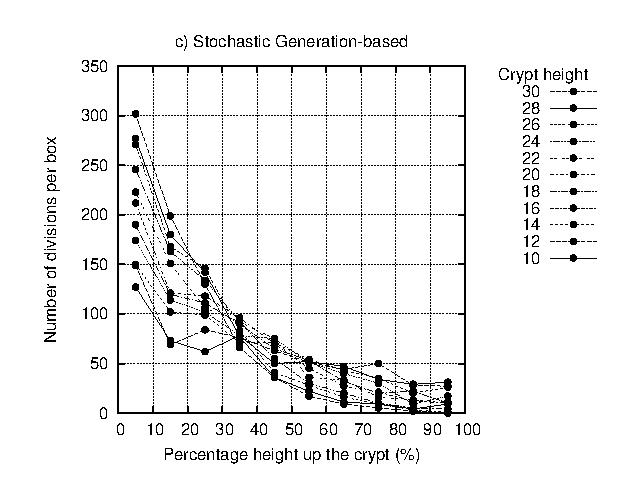
\includegraphics[width=.45\textwidth]{StochasticGenerationBased-Cell_division_locations}
\hspace*{5mm}
\includegraphics[width=.45\textwidth]{ContactInhibition-Cell_division_locations}
\end{center}
\end{frame}


\begin{frame}{Challenges arising}
\begin{itemize}
\item Setting `biological' parameters that don't have direct representations in all models
\item Describing the coupling of component models
\item Cell birth \& death imply non-regular result arrays
  \subitem{Move to ragged arrays as supported by HDF5, SciPy, etc.}
\item What post-processing should be in the protocol language?
  \begin{itemize}
  \item What is best as dedicated code or workflow?
  \item A language targeted at protocol exchange should be supportable by multiple tools
  \end{itemize}
  % Could talk about difference between prototyping something, and deposition in a standard format in a repository when a protocol is widespread/mature.
\end{itemize}
\end{frame}


%%%%%%%%%%%%%%%%%%%%%%%%%%%%%%%%%%%%%%%%%%%%%%%%%%%%%%%%%%%%%%%%%%%%%%
\section{Conclusions and future directions}
\subsection*{Main}
%%%%%%%%%%%%%%%%%%%%%%%%%%%%%%%%%%%%%%%%%%%%%%%%%%%%%%%%%%%%%%%%%%%%%%

\begin{frame}{Plans for this year}
\begin{itemize}
\item Comprehensive cardiac protocol suite
\item Summer intern working on Python implementation
\item Push SED-ML in the right direction
\item Parameter fitting (SED-ML, MSRC)
\end{itemize}
\end{frame}


\begin{frame}{Parameter estimation in SED-ML}
\begin{itemize}
\item Discussion document on \myhref{https://docs.google.com/document/d/1rrs0fYuKFr4fgL1b7eGwSnaLhRPW6NdXwAaJY0ZN_WY/edit}{Google Docs}
\item New kind of Task class for parameter estimation
  \begin{itemize}
  \item Algorithm referencing KiSAO, with parameters
  \item Objective function: least squares, MLE, \ldots
  \item Identify model parameters to be fit, with bounds/prior
    \subitem{And list of relevant experiments}
  \item Define the experiments to fit against
    \begin{itemize}
    \item Referencing data formats (dataSource)
    \item Mapping to simulated results (from dataGenerator)
    \item Weighting/scaling/error on data
    \end{itemize}
  \end{itemize}
\end{itemize}
\end{frame}


\begin{frame}{Feedback welcome}
\begin{itemize}
\item On the text syntax
\item On any extra features needed
\item On usability
\item On future directions
\end{itemize}
\end{frame}


\begin{frame}{Conclusions}
\begin{itemize}
\item Functional curation offers great scope for transforming our approach to modelling
\item Initial prototype is promising
\item Lots to do to demonstrate this fully
\end{itemize}
\end{frame}


\begin{frame}{Software Carpentry Workshop}
\begin{itemize}
\item 9-10 May 2013
\item For first and second year DTC students
\item Teaching basics of good scientific programming
  \begin{itemize}
  \item Python, SciPy, version control, testing, databases, doing it in Matlab
  \item Based on \myhref{http://software-carpentry.org/}{software-carpentry.org}
  \end{itemize}
\item Helpers required!
\end{itemize}
\end{frame}


%%%%%%%%%%%%%%%%%%%%%%%%%%%%%%%%%%%%%%%%%%%%%%%%%%%%%%%%%%%%%%%%%%%%%%
\begin{frame}{Acknowledgments}
Gary Mirams\\
Chaste team\\
Alan Garny, Steven Niederer, David Gavaghan

Reference publication: \doi{10.1016/j.pbiomolbio.2011.06.003}\\
Website: \myurl{https://chaste.cs.ox.ac.uk/trac/wiki/FunctionalCuration}

\begin{center}
\includegraphics[scale=.9]{chaste-266x60}\\ \vspace{.3cm}
\includegraphics[scale=.7]{logo2020science}\\ \vspace{.4cm}
\includegraphics[width=.55\textwidth]{EPSRC1RGBLO} \hspace{.1cm}
\includegraphics[scale=.55]{logo_msr}
\end{center}
\end{frame}


%%%%%%%%%%%%%%%%%%%%%%%%%%%%%%%%%%%%%%%%%%%%%%%%%%%%%%%%%%%%%%%%%%%%%%
\appendix


\begin{frame}{Name resolution}
\begin{center}
\vspace{-.5cm}
\includegraphics{Name_resolution}
\end{center}
\end{frame}


\end{document}
